% ------------------------------------------------------------------------------
% TYPO3 v9 LTS - What's New (English Version)
%
% @author	Michael Schams <schams.net>
% @license	Creative Commons BY-NC-SA 3.0
% @link		https://typo3.org/help/documentation/whats-new/
% @language	English
% ------------------------------------------------------------------------------

\section{Admin Panel}
\begin{frame}[fragile]
	\frametitle{Admin Panel}

	\begin{center}\huge{\color{typo3darkgrey}\textbf{Admin Panel}}\end{center}
	\begin{center}\large{\textit{An insight into the internal processes of TYPO3 at run-time}}\end{center}

\end{frame}

% ------------------------------------------------------------------------------
% Admin Panel

\begin{frame}[fragile]
	\frametitle{Admin Panel}
	\framesubtitle{Re-developed Admin Panel}

    The Admin Panel received a complete overhaul regarding its design as well as
    the underlying code and architecture.
	\newline\newline
	It is displayed at the bottom of a page in the frontend of TYPO3. The toggle
	button at the right allows integrators and editors to enable and disable the
	Admin Panel. The screenshot below shows the \textit{enabled} state.
	\vspace{0.8cm}
	\begin{figure}
		
\includegraphics[width=0.90\linewidth]{AdminPanel/AdminPanelEnabled.png}
	\end{figure}

\end{frame}

% ------------------------------------------------------------------------------
% Admin Panel: TypoScript Options

\begin{frame}[fragile]
	\frametitle{Admin Panel}
	\framesubtitle{Admin Panel: TypoScript Options}

	Example screenshot below shows TypoScript options.

	\begin{figure}
		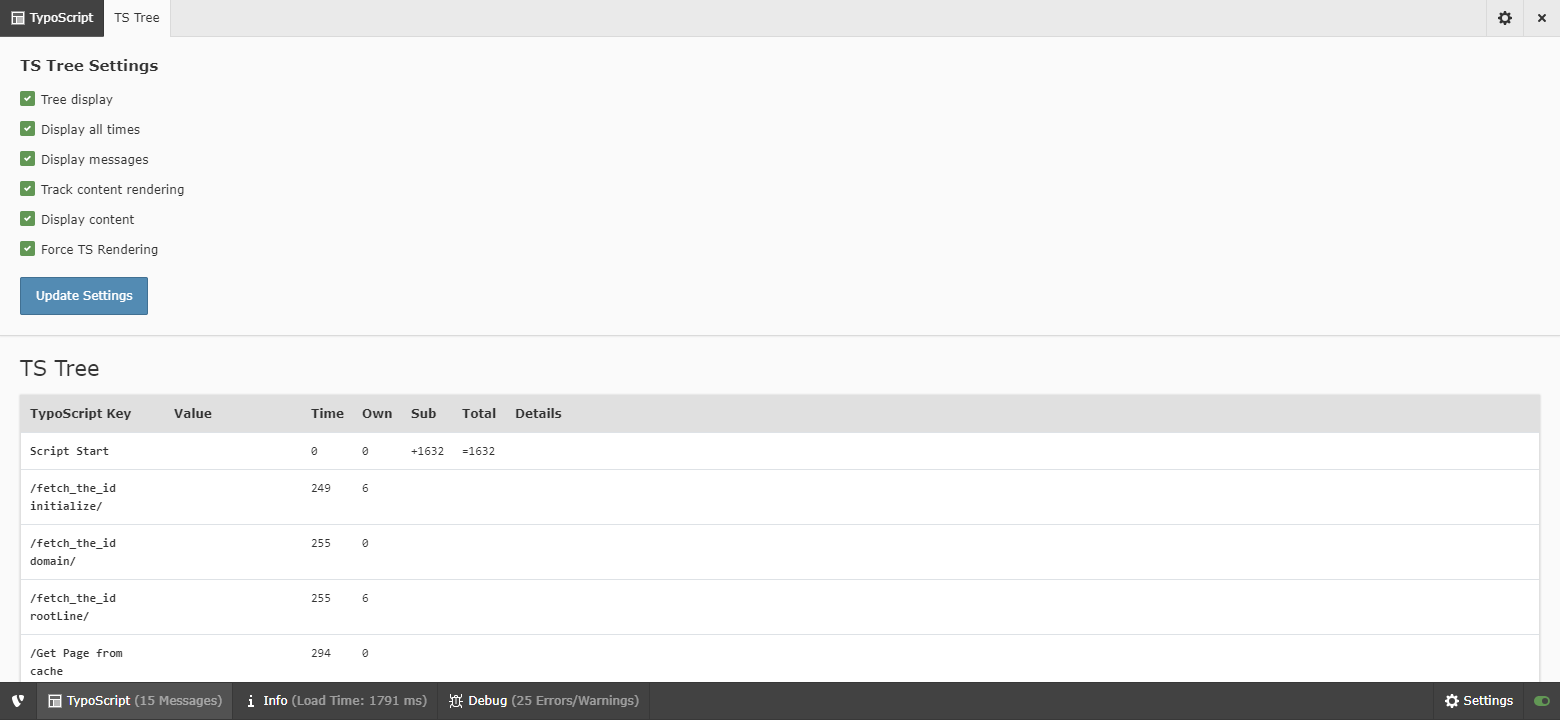
\includegraphics[width=0.90\linewidth]{AdminPanel/AdminPanelTypoScript.png}
	\end{figure}

\end{frame}

% ------------------------------------------------------------------------------
% Admin Panel: Configuration Options

\begin{frame}[fragile]
	\frametitle{Admin Panel}
	\framesubtitle{Admin Panel: Configuration Options}

	Example screenshot below shows configuration options ("Settings").

	\begin{figure}
		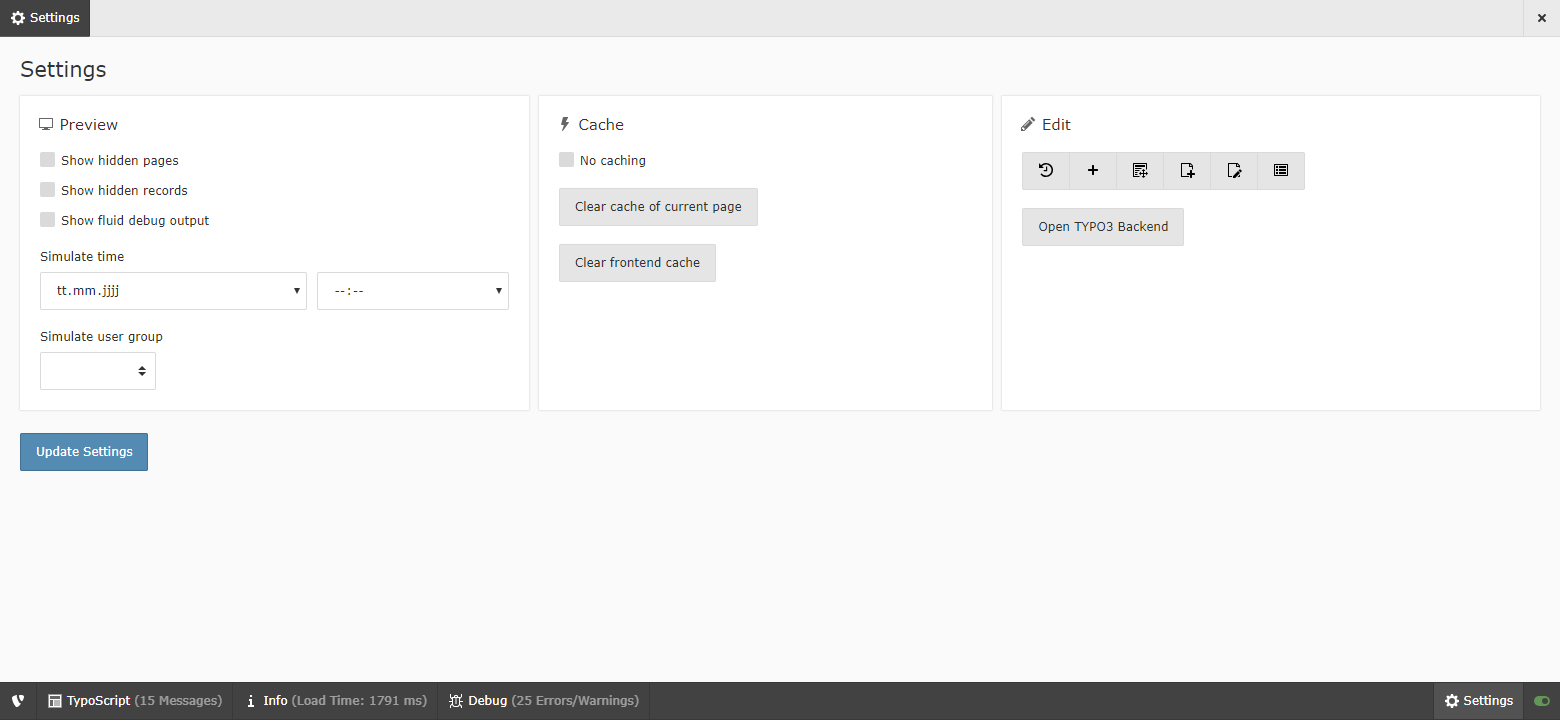
\includegraphics[width=0.90\linewidth]{AdminPanel/AdminPanelSettings.png}
	\end{figure}

\end{frame}

% ------------------------------------------------------------------------------
